\vspace*{-0.4cm}
\section{Introduction}
\label{section:introduction}




The database, HCI and systems communities have proposed tools that simplify common tasks of analytical processes. Such tools, however, either focus on only individual stages (such as data retrieval or visualization) of a much bigger analytical pipeline or they focus on particular use cases (for instance pattern matching, finding correlations and so on). Despite their remarkable success, data analysts often want the flexibility that comes from combining diverse tools and computation libraries in order to perform an analysis. This need often pushes code-literate data analysts to the tried-and-true interactive notebooks, such as Jupyter \cite{Jupyter}.


\begin{figure}[t]
  \centering
  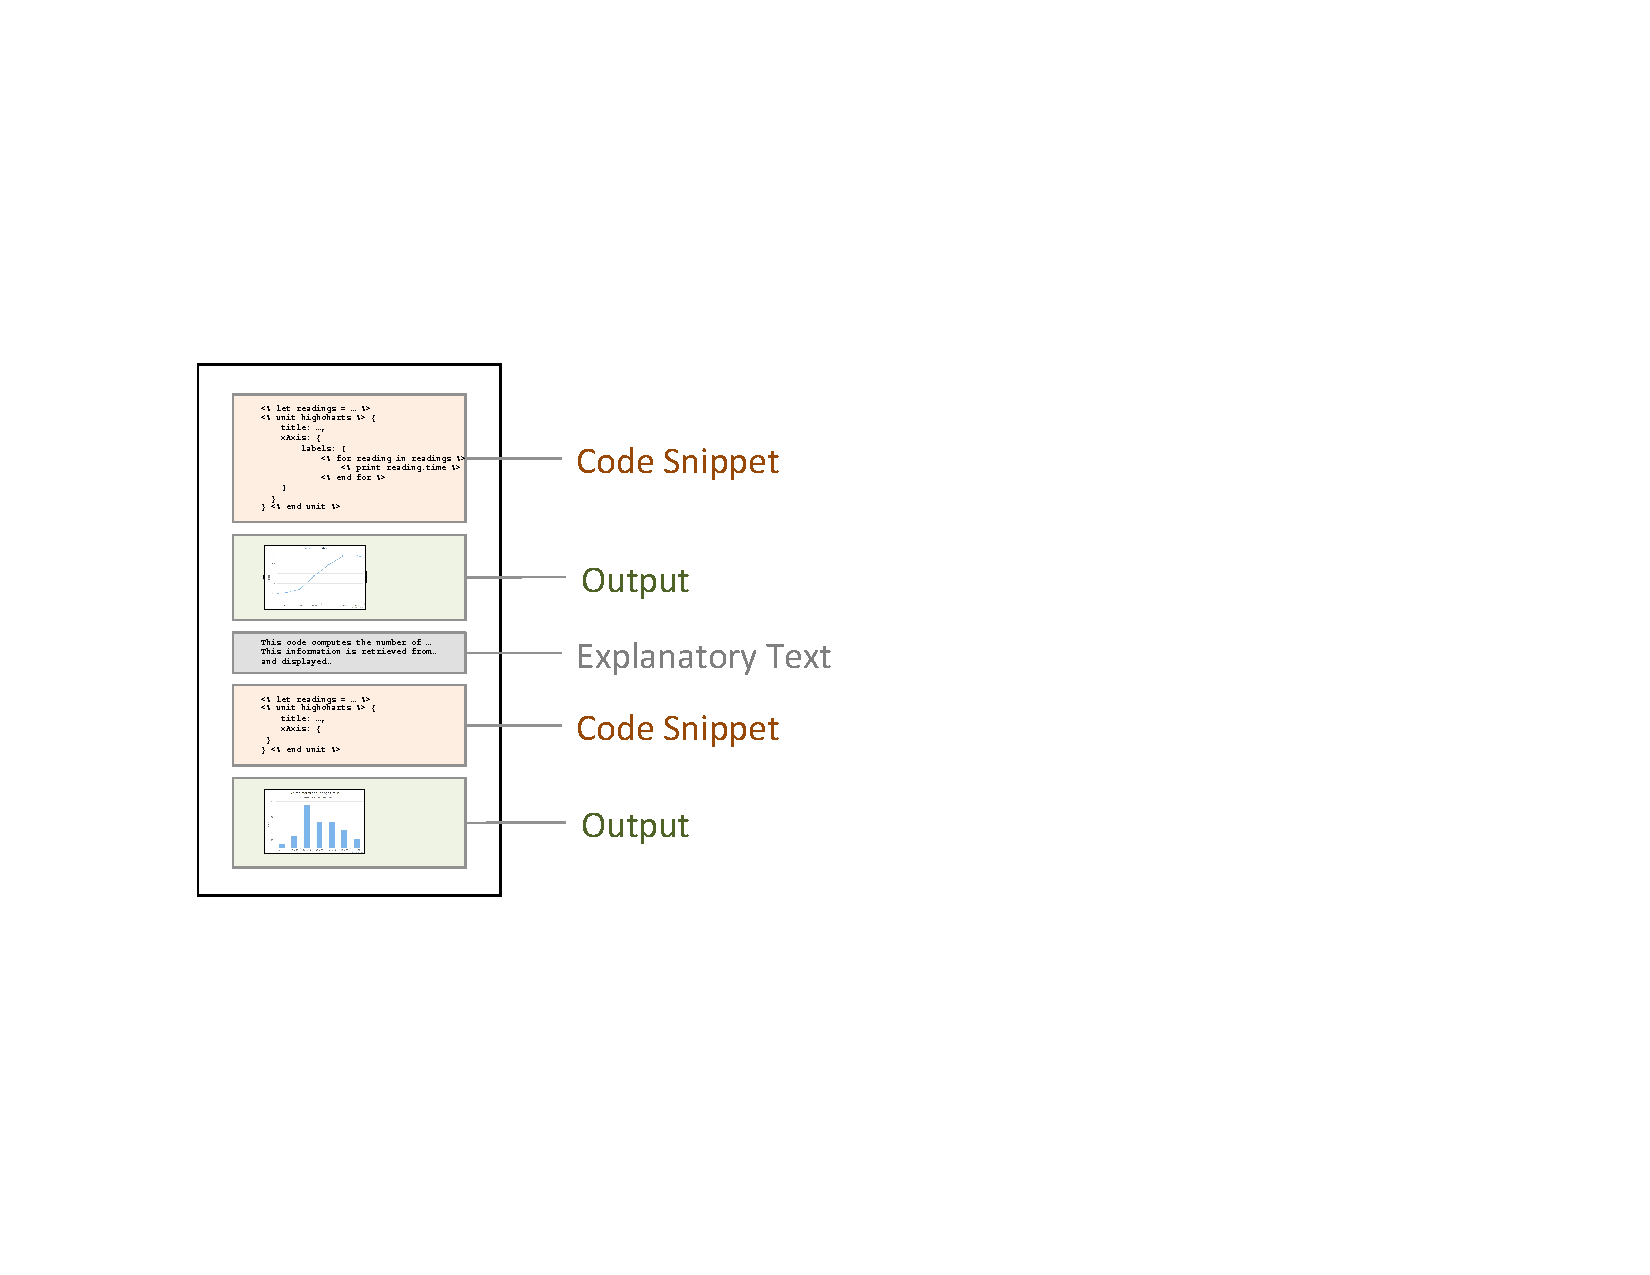
\includegraphics[width=0.7\columnwidth]{figures/notebook2.pdf}
  \caption{Notebook interface}
  \vspace{-15pt}
\label{figure:notebook-interface}
\end{figure}

Interactive notebooks allow the use of popular, highly expressive imperative languages, such as Python, for describing tasks such as data retrieval, processing and visualization, all in one platform. Due to the popularity of the languages they support, there is a massive collection of third-party utility libraries that can be used to facilitate such tasks. Furthermore, the web environment of interactive notebooks enables collaboration between data analysts, since it allows them to develop and run code that processes data and generates visualizations directly on the browser. Lastly, after completing an analysis, data analysts can compose their findings into an interactive report-like page, that contains re-runnable code, visualizations and textual description of the analysis, which can also be shared with non-technical users. Figure \ref{figure:notebook-interface}, shows the interface of Jupyter notebooks. It comprises a sequence of blocks that are created ``on-demand" by the data analyst, each block can contain explanatory text and re-runnable coding snippets that once evaluated print the result (which could be a visualization or plain text) into the subsequent block. 
%For those reasons, notebooks are extensively used in data science projects.


\eat{
However, interactive notebooks are still suboptimal with regard to ease of use and productivity for data analysts. 
Retrieving, processing and visualizing data requires technical expertise that often exceeds the skill-set of a typical data analyst. Specifically, such steps require data transfers and package installations on the notebook server, in order to be used in an analysis. Such tasks fit the job description of a system administrator rather than a data analyst. \costas{downplay the sysadmin aspects of it.} Additionally, even after the environment has been setup, the data analyst has to read long documentation files that explain how to programmatically interact with such tools and she often has to spend significant effort writing plumbing code in order combine their functionality.
}

However, interactive notebooks are still suboptimal with regard to ease of use and productivity for data analysts. Retrieving, processing and visualizing data involves reading lengthy documentation pages that describe each library's programmatic API and writing complex imperative plumbing code in order combine their functionality. Both these steps, are not only very time consuming but also require technical expertise that exceeds the skill-set of a typical data analyst. 



Besides the aforementioned limitations that impact data analysts, notebooks also have limitations that impact the, potentially non-technical, readers of the published notebooks. Particularly, while notebooks can contain visualizations that showcase important aspects of a data analysis, the readers cannot interact with the provided visualizations in the same way they could if these visualizations were part of a typical OLAP dashboard application. Specifically, even if the analyst that composed the notebook used third-party web-based visualization libraries that support user interaction, this interaction can only cause local changes to the visualization the reader interacts with and cannot trigger additional data retrieval, computation or mutations to other visualizations that are included in the notebook. For this reason, only code-literate readers, capable of extending the notebook with more coding snippets, are able to further explore the underlying data (or examine additional hypotheses about the underlying data), while the rest are limited to passively reading the generated notebook.

\costas{Does this point belong to both the reader and the data analyst of the notebook? Regardless of the techinical expertise of the analyst, building an OLAP-like dashboard just cannot be done in a notebook.}


\noindent {\bf Contributions.}
In order to resolve these issues, we extend Jupyter interactive notebooks with the  {\projname} notebook engine. The main contributions of this extension are: (a) visual and data retrieval constructs, that simplify the process of data retrieval and visualization, for data analysts, (b) A declarative template language that can be used to declaratively describe computation, data transformations, user input collection, (c)\eat{an easy to use API that allows wrapping existing Python coding blocks into reusable functions that can be employed in the template to describe data process and (d) }A propagation algorithm, capable of propagating changes from visual and data retrieval constructs to subsequent such constructs and Python coding blocks, thus introducing a truly reactive behavior to notebooks. These reactive capabilities, enable non-technical, code illiterate  readers to further explore the underlying data.

\eat{
\begin{compact_enum} 
\item visual and data retrieval constructs, that simplify the process of data retrieval and visualization, for data analysts, 
\item A declarative template language that can be used for describing computation, data transformations and user input collection, \eat{\yannis{shouldn't this item be bigger? It's not just input collection: doesn't it also define control flow?}}
\item A propagation algorithm, that utilizes visual and data retrieval constructs, combined with templates in order to introduce a reactive behavior to notebooks. These reactive capabilities, enable non-technical readers to further explore data, without requiring any coding skills. 
\end{compact_enum}
}
\eat{
The remainder of this paper is organized as follows: Section ?? discusses the architecture of the {\projname} framework. Due to space limitation, we focus on those aspects that can be useful as a notebook extension. Section ?? presents our example data analysis. Finally, Section ?? concludes the paper.
}

\eat{
\noindent {\bf Contributions.}
To sum up, we extend interactive notebooks with the  {\projname} notebook engine. The main contributions of this extension are: (a) visual and data retrieval constructs, that simplify the process of data retrieval and visualization, (b) A declarative template language that can be used for specifying computation, data transformations and user input collection, (c) A propagation algorithm, that utilizes visual and data retrieval constructs, in association with a template language in order to introduce a reactive in notebooks. 
}
\eat{

\begin{itemize}
	\item \textit{Expressive template language:} Prior work, treats a page as a database view. Building on that, our template language goes beyond SQL query and view definition in both style and fundamental expressiveness. It is a mixture of query as well as web templating language that works on ordered (arrays) and semi-ordered (JSON) data. 
	\item \textit{Easy data retrieval:} Our framework supports communication with all major database types, such as Postgress, MongoDB, SQL etc, eliminating the need for individual DB drivers. Furthermore, using {\projname}, user access credentials for the database server(s) are stored in a configuration file, eliminating the embarassingly insecure practice of typing usernames and passwords in notebook cells vidible to everyone.
	\item \textit{Inline JSON operations:} The primary data structure used in {\projname} is JSON arrays. {\projname} combines the intuitive nature of JSON with the ability to write inline JSON operations, resulting in a clean, structured and readable code.
	\item \textit{Variable binding:} Analysts can easily ``bind'' variables using our template language. ``Binding'', results in automatic re-execution of notebook cells that contain those variables upon a change. {\projname} will trigger execution of the appropriate cells without any extra coding effort. As we show later, combined with inline JSON operations, binding becomes an incredibly versatile tool.

%	\item \textit{Declarative semantics:} {\projname} implements formal declarative \textit{Model-View-View-Model} (MVVM) semantics. \remark{Fill in why this is a good thing. I have no idea.}
%	\item \textit{Expressive template language:} Prior database work, treats a page as a database view. Building on that, our template language goes beyond SQL query and view definition in both style and fundamental expressiveness. It is a mixture of query as well as web templating language that works on ordered (arrays) and semi-ordered (JSON) data. 
%	\item We allow in-line declarative code directly in JSON...
\end{itemize}

}


\eat{
\begin{figure*}
	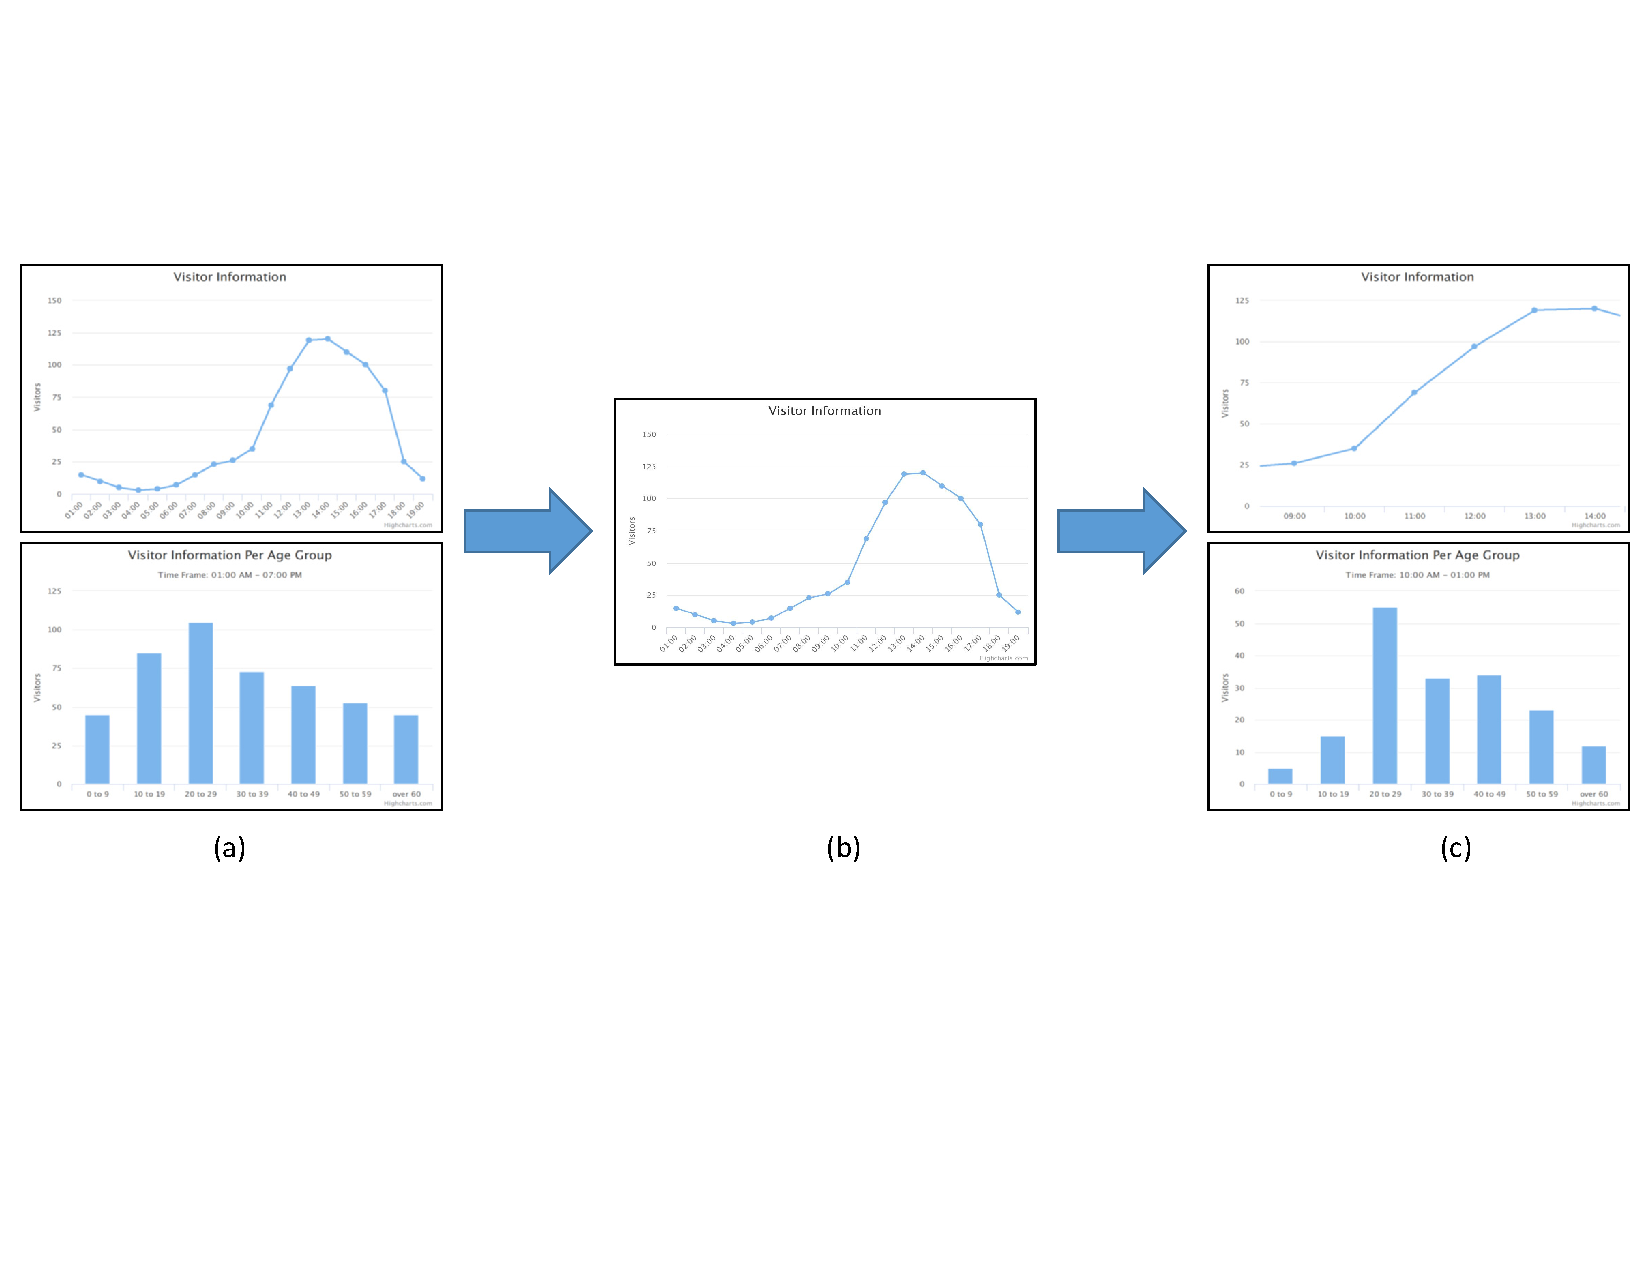
\includegraphics[width=\textwidth]{figures/highchart_final_a.pdf}
	\caption{Demonstration of interactive charts. The analyst's selection automatically updates the second plot (right).}
	\label{fig:vision}
\end{figure*}
}
\eat{
\begin{figure*}
	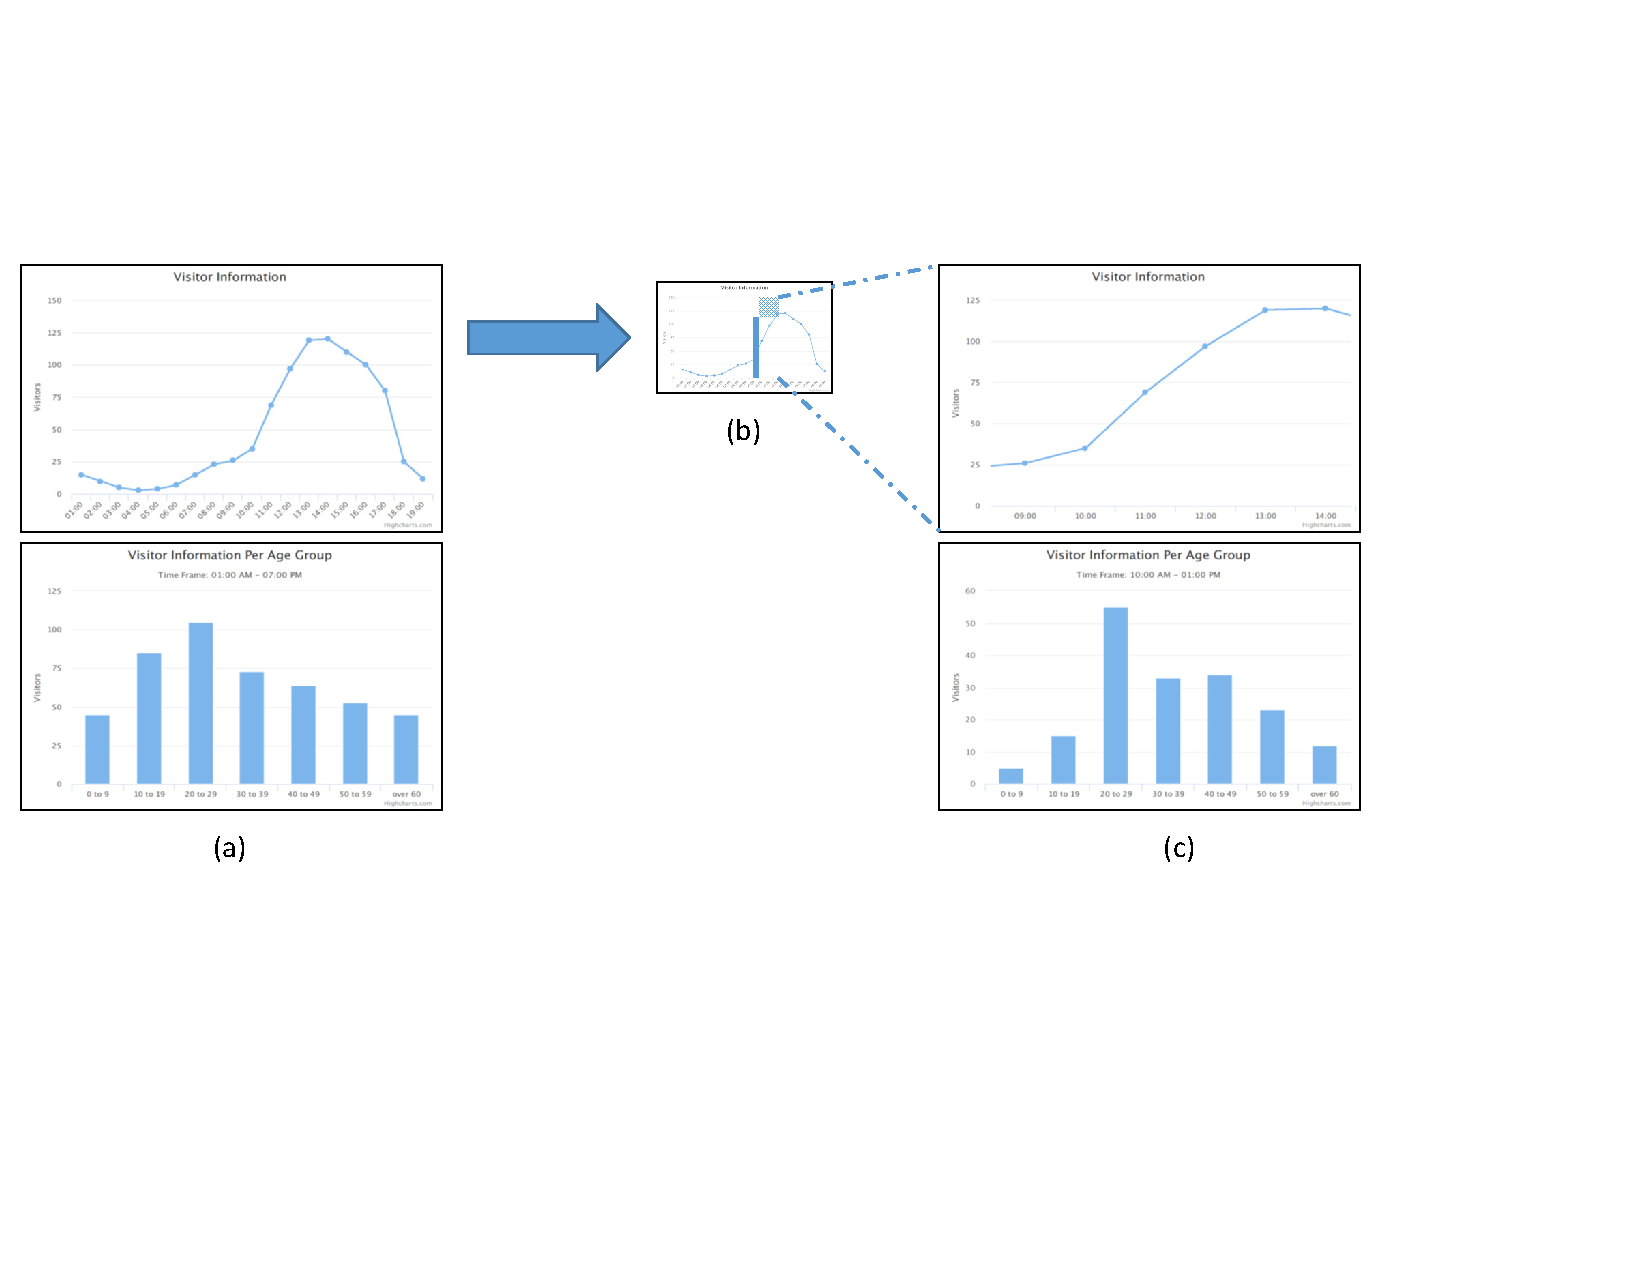
\includegraphics[width=\textwidth]{figures/highchart_final_b.pdf}
	\caption{Demonstration of interactive charts. The analyst's selection automatically updates the second plot (right).}
	\label{fig:vision}
\end{figure*}
}
\eat{
\remark{Ok I thought about it and I propose the following modifications in the paper structure (Nothing major - just moving text around to make it more readable): We begin with a good discussion about the vidette features that can help notebooks in section 2. We then show the entire walkthrough in one section (Section 3). By now, the reader knows what vidette can do so it will be easier to follow and understand the code we show.}
}
 \eat{
We address these issues, by extending interactive notebooks with the  {\projname} framework. {\projname} notebooks support a new template language capable of facilitating common data analysis tasks. The main contributions of this extension are:

\begin{itemize}
	\item \textit{Expressive template language:} Prior work, treats a page as a database view. Building on that, our template language goes beyond SQL query and view definition in both style and fundamental expressiveness. It is a mixture of query as well as web templating language that works on ordered (arrays) and semi-ordered (JSON) data. 
	\item \textit{Easy data retrieval:} Our framework supports communication with all major database types, such as Postgress, MongoDB, SQL etc, eliminating the need for individual DB drivers. Furthermore, using {\projname}, user access credentials for the database server(s) are stored in a configuration file, eliminating the embarassingly insecure practice of typing usernames and passwords in notebook cells vidible to everyone.
	\item \textit{Inline JSON operations:} The primary data structure used in {\projname} is JSON arrays. {\projname} combines the intuitive nature of JSON with the ability to write inline JSON operations, resulting in a clean, structured and readable code.
	\item \textit{Variable binding:} Analysts can easily ``bind'' variables using our template language. ``Binding'', results in automatic re-execution of notebook cells that contain those variables upon a change. {\projname} will trigger execution of the appropriate cells without any extra coding effort. As we show later, combined with inline JSON operations, binding becomes an incredibly versatile tool.

%	\item \textit{Declarative semantics:} {\projname} implements formal declarative \textit{Model-View-View-Model} (MVVM) semantics. \remark{Fill in why this is a good thing. I have no idea.}
%	\item \textit{Expressive template language:} Prior database work, treats a page as a database view. Building on that, our template language goes beyond SQL query and view definition in both style and fundamental expressiveness. It is a mixture of query as well as web templating language that works on ordered (arrays) and semi-ordered (JSON) data. 
%	\item We allow in-line declarative code directly in JSON...
\end{itemize}
}


%In this paper, we demonstrate the use of {\projname} via a walkthrough example. Specifically, we want to use website access data to plot an access count over time histogram. We also want to plot the recorded user demographics (with focus on age groups). We then want to have the ability to interact with the histogram plot and select a time region. This action should automatically update the second plot with the user demographics in the selected time window. 
%
%Without loss of generality, we assume a Jupyter server, where the analysts develop their notebooks and a different database server where data is stored. To retrieve the entirety of the required data, we have to query two different databases and join the returned JSON files. Figure ?? shows how our databases are organized. Our fictional analyst will perform the following high-level tasks:
%
%\begin{itemize}
%	\item Data retrieval from remote databases. 
%	\item Data curation: Join data and prepare for visualization.
%	\item Data visualization.
%\end{itemize}
%
%The remainder of this paper is organized as follows: Sections \ref{section:dataretrieval} -- \ref{section:visualization} present a direct comparison of using {\projname} and an imperative language such as Python in order to complete the tasks of our example. Throughout these sections, we demonstrate some of the main contributions of {\projname}. Section \ref{section:discussion} provides further discussion regarding our proposed extension and presents other useful aspects of it not used in our walkthrough. Finally, Section \ref{section:conclusion} concludes the paper.

